
The block diagram for the inner loop is shown in Figure~\ref{fig:hw_ballbeam_system_type_inner}.
\begin{figure}[H]
   \centering
   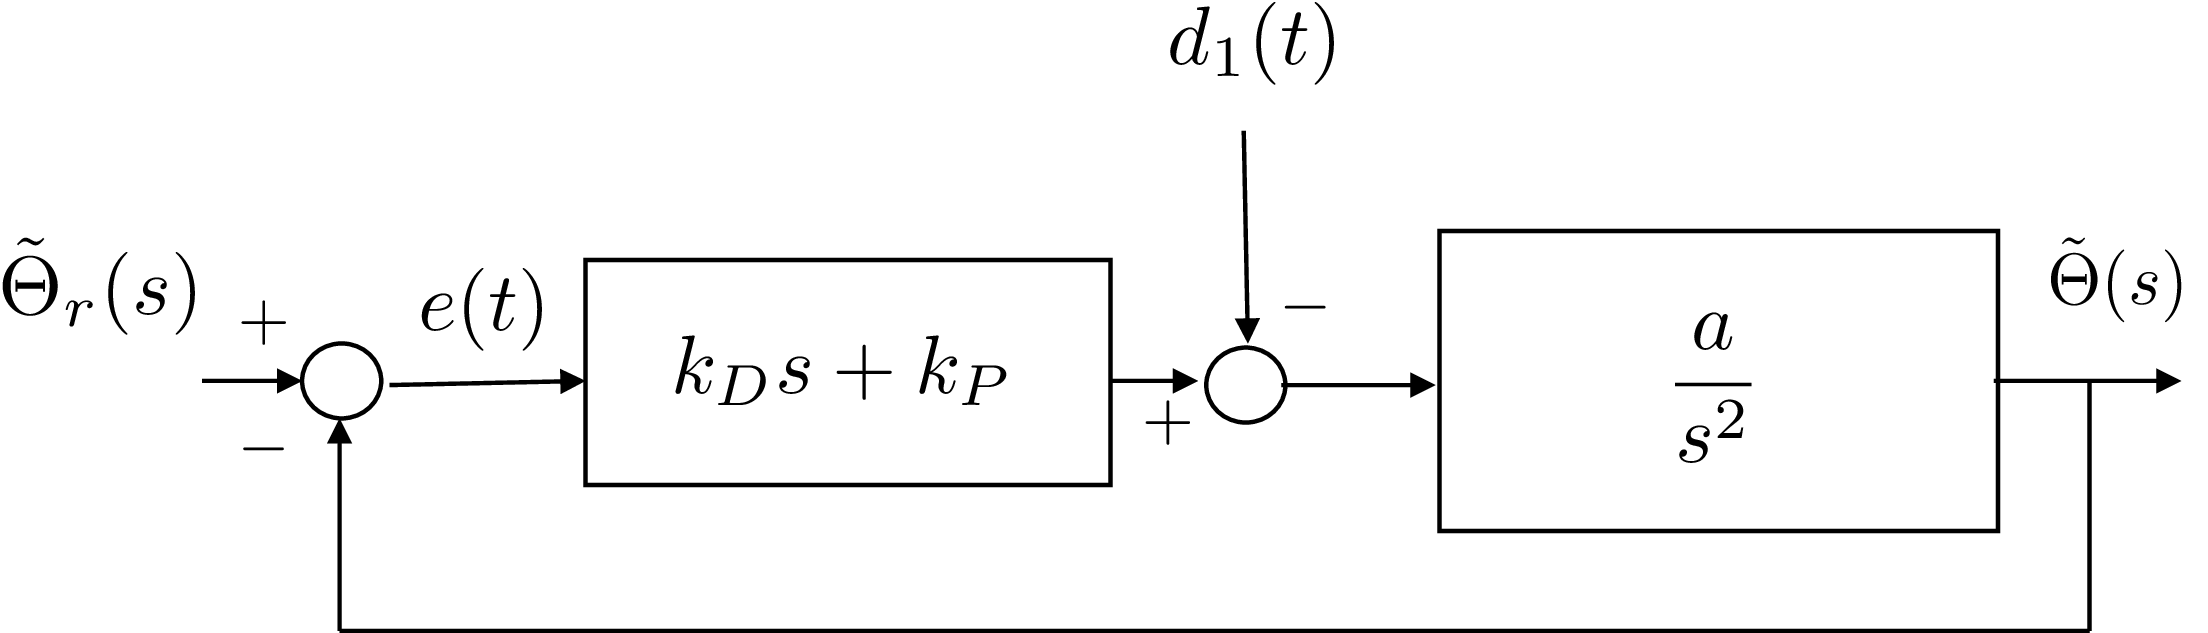
\includegraphics[width=0.8\textwidth]{6_design_studies/figures/hw_ballbeam_system_type_inner.pdf}
   \caption{Inner loop system for problem HW~\ref{hw:ballbeam}.\ref{chap:PID-system-type}.}
   \label{fig:hw_ballbeam_system_type_inner}
\end{figure}
The open loop system is given by
\[
P(s)C(s) = \left(\frac{a}{s^2}\right)\left(k_Ds+k_P\right),
\]
where
\[
a \defeq \frac{\ell}{\frac{m_2\ell^2}{3}+m_1z_e^2}.
\]
Since there are two free integrators, the system is type~2, and from Table~\ref{table:system_type} the tracking error when the input is a step or ramp is zero, and when it is a parabola
\[
\lim_{t\to\infty}e(t) = \frac{1}{M_a} = \frac{1}{\lim_{s\to 0} s^2P(s)C(s)} = \frac{1}{ak_P}.
\]

The transfer function from $d(t)$ to $e(t)$ is
\begin{align*}
E(s) &= \frac{P(s)}{1+P(s)C(s)}D(s) \\
     &= \frac{\frac{a}{s^2}}{1+\left(\frac{a}{s^2}\right)(k_D s+k_P)}D(s) \\
     &= \frac{a}{s^2+ak_Ds+ak_P}D(s).
\end{align*}

For the disturbance input, the steady state error to a step on $d(t)$ is
\begin{align*}
\lim_{t\to\infty}e(t) &= \lim_{s\to 0}s\frac{P(s)}{1+P(s)C(s)}\frac{1}{s} \\
&= \lim_{s\to 0} \frac{a}{s^2+ak_Ds+ak_P} = \frac{1}{k_P}.
\end{align*}
Therefore, the system is type~0 with respect to the input disturbance.

The block diagram for the outer loop is shown in Figure~\ref{fig:hw_ballbeam_system_type_outer}.
\begin{figure}[H]
   \centering
   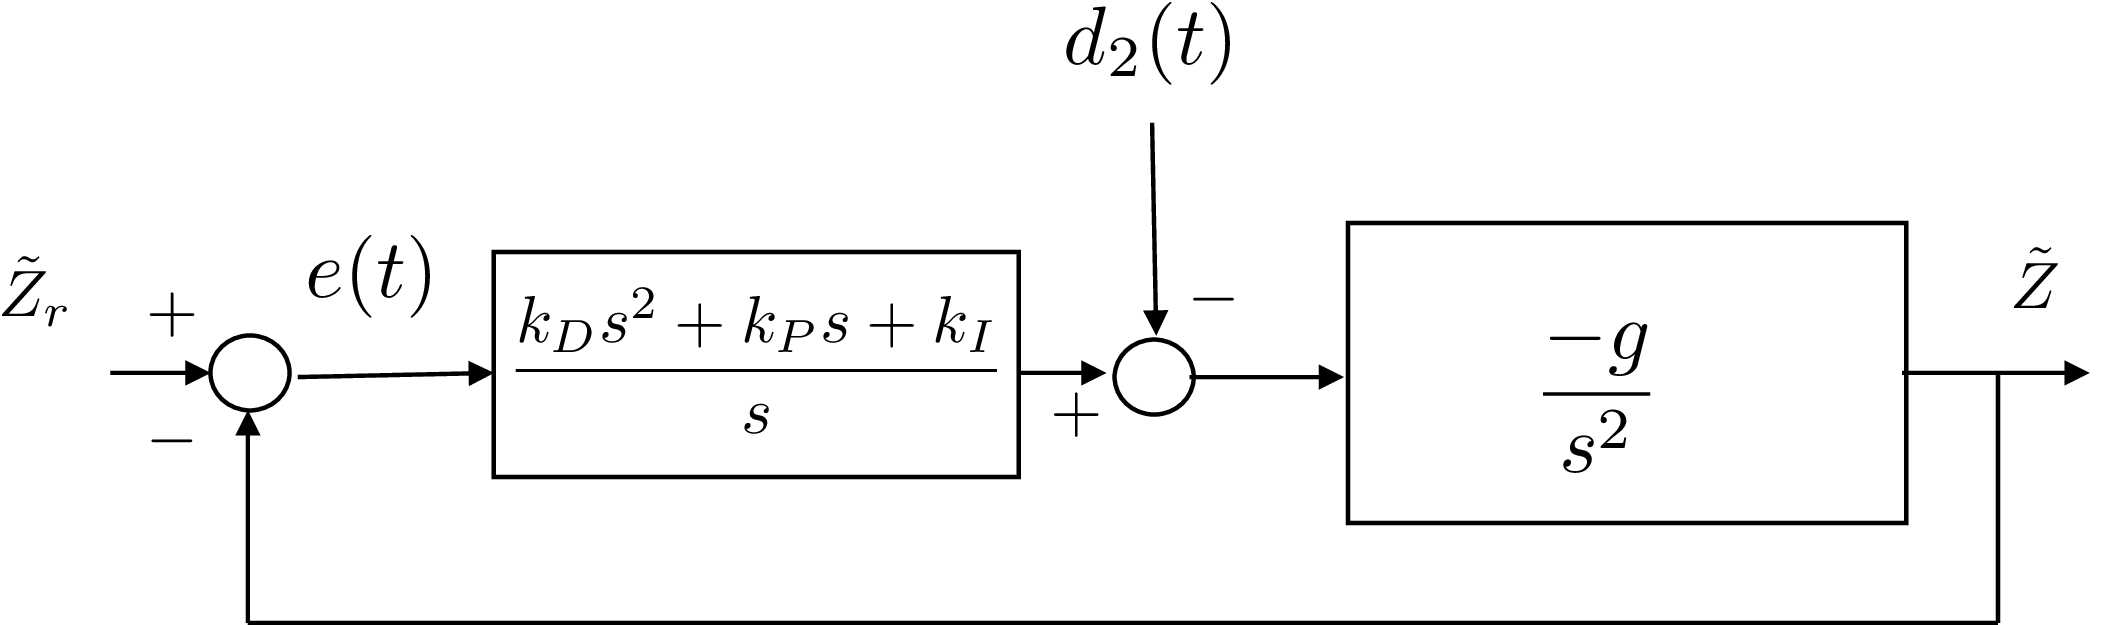
\includegraphics[width=0.8\textwidth]{6_design_studies/figures/hw_ballbeam_system_type_outer.pdf}
   \caption{Outer loop system for problem HW~\ref{hw:ballbeam}.\ref{chap:PID-system-type}.}
   \label{fig:hw_ballbeam_system_type_outer}
\end{figure}
The open loop system is given by
\[
P(s)C(s) = \left(\frac{-g}{s^2}\right)\left(\frac{k_Ds^2+k_Ps+k_I}{s}\right).
\]
When $k_I=0$ there are two free integrator in $P(s)C(s)$ and the system is type~2, and from Table~\ref{table:system_type} the tracking error when the input is a parabola is \[
\lim_{t\to\infty}e(t) = \frac{1}{M_a} = \frac{1}{\lim_{s\to 0} s^2P(s)C(s)} = -\frac{1}{gk_P}.
\]
When $k_I\neq 0$, there are three free integrators in $P(s)C(s)$ and the system is type~3.  From Table~\ref{table:system_type} the tracking error when the input is $t^3$ is 
\[
\lim_{t\to\infty}e(t) = \frac{1}{\lim_{s\to 0} s^3P(s)C(s)} =- \frac{1}{gk_I}.
\]

For the disturbance input, the steady state error when $D(s) = \frac{1}{s^{q+1}}$ is
\begin{align*}
\lim_{t\to\infty}e(t) &= \lim_{s\to 0}\frac{sP(s)}{1+P(s)C(s)}\frac{1}{s^{q+1}} \\
					  &= \lim_{s\to 0} \frac{\frac{-g}{s^2}}{1+\left(\frac{-g}{s^2}\right)\left(\frac{k_Ds^2+k_Ps+k_I}{s}\right)}\frac{1}{s^q} \\
					  &= \lim_{s\to 0} \frac{-gs}{s^3+(-gk_D)s^2+(-gk_P)s + (-gk_I)}\frac{1}{s^q}.					  
\end{align*}
Without the integrator, i.e., when $k_I=0$ we have
\begin{align*}
\lim_{t\to\infty}e(t) &= \frac{1}{k_P}\frac{1}{s^q}
\end{align*}
which is finite when $q=0$.  Therefore, the system is type~0 with respect to the input disturbance and the steady state error when $d_2(t)$ is a unit step is $1/k_P$.  

When $k_I\neq 0$, we have
\begin{align*}
\lim_{t\to\infty}e(t) &= \frac{1}{k_I}\frac{1}{s^{q-1}}
\end{align*}
which is finite when $q=1$.  Therefore, the system is type~1 with respect to the input disturbance and the steady-state error when $d_2(t)$ is a unit ramp is $1/k_I$.  

